%
% File acl2019.tex
%
%% Based on the style files for ACL 2018, NAACL 2018/19, which were
%% Based on the style files for ACL-2015, with some improvements
%%  taken from the NAACL-2016 style
%% Based on the style files for ACL-2014, which were, in turn,
%% based on ACL-2013, ACL-2012, ACL-2011, ACL-2010, ACL-IJCNLP-2009,
%% EACL-2009, IJCNLP-2008...
%% Based on the style files for EACL 2006 by 
%%e.agirre@ehu.es or Sergi.Balari@uab.es
%% and that of ACL 08 by Joakim Nivre and Noah Smith

\documentclass[11pt,a4paper]{article}
\usepackage[hyperref]{acl2019}
\usepackage{times}
\usepackage{latexsym}
\usepackage{amsmath}
\usepackage{amsfonts}
\usepackage{graphicx}
\usepackage{caption}
\usepackage{subcaption}
\usepackage{hyperref}

\usepackage{relsize}
\renewcommand*{\UrlFont}{\smaller\relax}


\DeclareMathOperator*{\argmax}{arg\,max}
\DeclareMathOperator*{\argmin}{arg\,min}
\usepackage{enumitem}


\usepackage{url}

\aclfinalcopy % Uncomment this line for the final submission
%\def\aclpaperid{***} %  Enter the acl Paper ID here

%\setlength\titlebox{5cm}
% You can expand the titlebox if you need extra space
% to show all the authors. Please do not make the titlebox
% smaller than 5cm (the original size); we will check this
% in the camera-ready version and ask you to change it back.
\newcommand\BibTeX{B\textsc{ib}\TeX}

\title{Concept Tagging for the Movie Domain by using Transfer Learning and Named Entity Recognition.}

\author{Giovanni De Toni (197814) \\
  University of Trento \\ Via Sommarive, 9, 38123 Povo,Trento TN\\
  \texttt{giovanni.detoni@studenti.unitn.it}}

\date{}

\begin{document}
\maketitle

\begin{abstract}
Neural Networks have produced remarkable results in many Natural Language Processing tasks, for example, when tasked to assigning concepts to words of a sentence. Their successes are made possible by employing good word representations (embeddings) which a Neural Network can understand. This work evaluates several newly developed pre-trained embeddings (ELMo, BERT and ConceptNet) on the task of tagging sequences from the movie domain. We then compare the measurements with previous results of the literature.
\end{abstract}

\section{Introduction}
Concept Tagging sequences is a classical problem in 
the NLP field. It consists of assigning to each word 
of a sentence a given concept which represents the 
meaning of that word (e.g., ``\textit{star wars}" is 
a movie title, hence the concept ``
\textit{movie.title}"). Over the past years, it was 
extensively studied and several techniques were 
developed such to efficiently tag words given a pool 
of concepts. The most basic methods are statistical 
language models (e.g., Weight Finite State Transducers) 
which are easy to train and yield quite impressive 
results with a little tuning. However, with the rise 
of Recurrent Neural Networks, we can now develop 
models which have better performances than their 
statistic counterparts. Moreover, thanks to the use 
of specific word embeddings (e.g., word2vec, GloVe, 
ELMo etc.), we can boost the performances even more.
This work takes as a starting point a previous paper 
on the topic by \citet{gobbi} and tries to improve 
the results of some of the neural models presented 
by adding new features (NER and POS tags) and 
by trying to employ more intelligent embeddings 
(ELMo, BERT and ConceptNet). We conducted several experiments with a few selected architectures and we tried to outperform the performances presented (with respect also to the classical WFST methods). The report is structured as follows: the second section describes 
the models used for the experiments, the third section gives a brief explanation about the possible types of embeddings and then it describes the chosen embeddings for our project. The fourth section describes the analysis of the 
dataset and of the embeddings. Ultimately, the fifth
and the sixth sections report the experiments 
performed and the discussion over the results.

\section{Models}

To evaluate how the performance changes with respect 
to the previous results we selected two models from 
the original work. We concentrated on the Neural 
Networks approaches by selecting the ones which held 
the best results over the test set. We chose the 
following architectures: LSTM and LSTM-CRF.  
Moreover, we extended the features used by the 
various models by providing also the \textbf{Part-of-Speech 
tags (POS)} and the \textbf{Named Entities Recognition (NER)} 
entities as one-hot-encoded vectors. We now describe the two selected architectures.

\textbf{Long-Short Term Memory (LSTM)} \cite{lstm} is a model 
which extends and improve the previous RNN by 
solving the vanishing/exploding gradients problem. 
We tested a simple LSTM which receives in input the 
embeddings of the words. Moreover, we tested another LSTM model which uses also the characters embeddings (CHAR) obtained using a convolutional layer concatenated with the new features. 

We experimented also with the \textbf{LSTM-CRF} model \cite{
yao2014recurrent, DBLP:journals/corr/HuangXY15} in 
which the LSTM provides the class scores for each 
token and then the Viterbi algorithm is used to 
determine the labels at a global level. Moreover, an 
LSTM-CRF version extended with the character 
embeddings and the new features was also evaluated.

\section{Embeddings}

As a first step to improve the performances of the previous work we concentrated on evaluating several recently proposed pre-trained language models to produce words representations.

Generally speaking, language representations can be either \textbf{context-free} or \textbf{contextual}. 
Context-free means that the word representation is generated without looking at the context in which the word is used. For instance, the word ``\textit{season}" may have different meanings with respect to the context in which it is placed (e.g., ``\textit{Summer is my favourite season}" and ``\textit{Season the chicken and then serve}"), but in a context-free model it will get the same representation (embedding). A contextual representation takes care also of the context in which a word is used.
Moreover, the contextual representations can be further divided into two other categories: unidirectional or bidirectional. 

A \textbf{unidirectional model} contextualizes a given term by just looking at the words on the right (or on the left) of it.  

A \textbf{bidirectional model} looks both on the left and on the right of the target word before producing a representation. There are also \textbf{shallow bidirectional models} which combine two unidirectional models (one for the left side and one for the right side) to give a more complete representation. In our work, we tested three different embeddings, one for each category (context-free, contextual shallow bidirectional and contextual bidirectional): ConceptNet, ELMo and BERT. We then compared their performances against the one used in the original work called \textbf{w2v\_trimmed} (a standard word2vec representation).

\subsection{ConceptNet}
\textbf{ConceptNet Numberbatch} \cite{speer2017conceptnet} is a context-free language representation. It is a set of word embeddings and it was made by combining previously existing models, namely: GloVe \cite{pennington2014glove}, word2vec \cite{mikolov2013efficient} and OpenSubtitles 2016 \cite{Lison2016OpenSubtitles2016EL}. Moreover, it leverages the data of the ConceptNet knowledge graph to enrich its representation. The authors reached this goal by using a retrofitting procedure to adjust the word embedding matrix by using their knowledge graph. Thanks to this procedure, ConceptNet is also intrinsically multilingual since this method pushes the model to use the same embedding space both for English words and words in different languages (since they share the same meaning).  This work uses the Numberbatch 19.08 English-only model \footnote{\url{https://github.com/commonsense/conceptnet-numberbatch}} which contains 516782 embeddings with a dimension of 300.

\subsection{ELMo}
\textbf{ELMo (Embeddings from Language Models)} \cite{Peters:2018} is a deep contextualized word representation which captures both syntactic, semantic and polysemy characteristics of a given word. It uses a deep shallow bidirectional language model (biLM) trained on a large corpus by looking at the entire input sentences. The generated representations are deep because they are a function of all the layers of the biLM. Moreover, each layer models certain features of the given word. The original work states that the higher-level LSTM layers capture context-dependent aspects of the word meaning, while lower-level states capture aspects of the syntax.
We used the pre-trained small ELMo model \footnote{\url{https://allennlp.org/elmo}} with the embedding dimension of 1024.
In this work, the the final embeddings were produced by \textbf{linear combination} from the ELMo hidden layers. If $\mathbf{h_i}$ denotes an ELMo hidden layer, the final embeddings $\mathbf{e}$ can be computed by doing $\mathbf{e} = \sum_{i=0}^{N} \mathbf{h_i} \cdot w_i$, where $N$ is the number of layers. We devised two strategies to estimate the scalar weights $w_i$:
\begin{itemize}[noitemsep]
\item \textbf{Averaged}: $w_i = \frac{1}{N}$ to give an equal weighting; 
\item \textbf{Fine-tuned}: it learns directly all $w_i$ during the training of the final concept tagger.
\end{itemize}

\begin{figure*}[t]
\begin{subfigure}{0.5\linewidth}
  \centering
  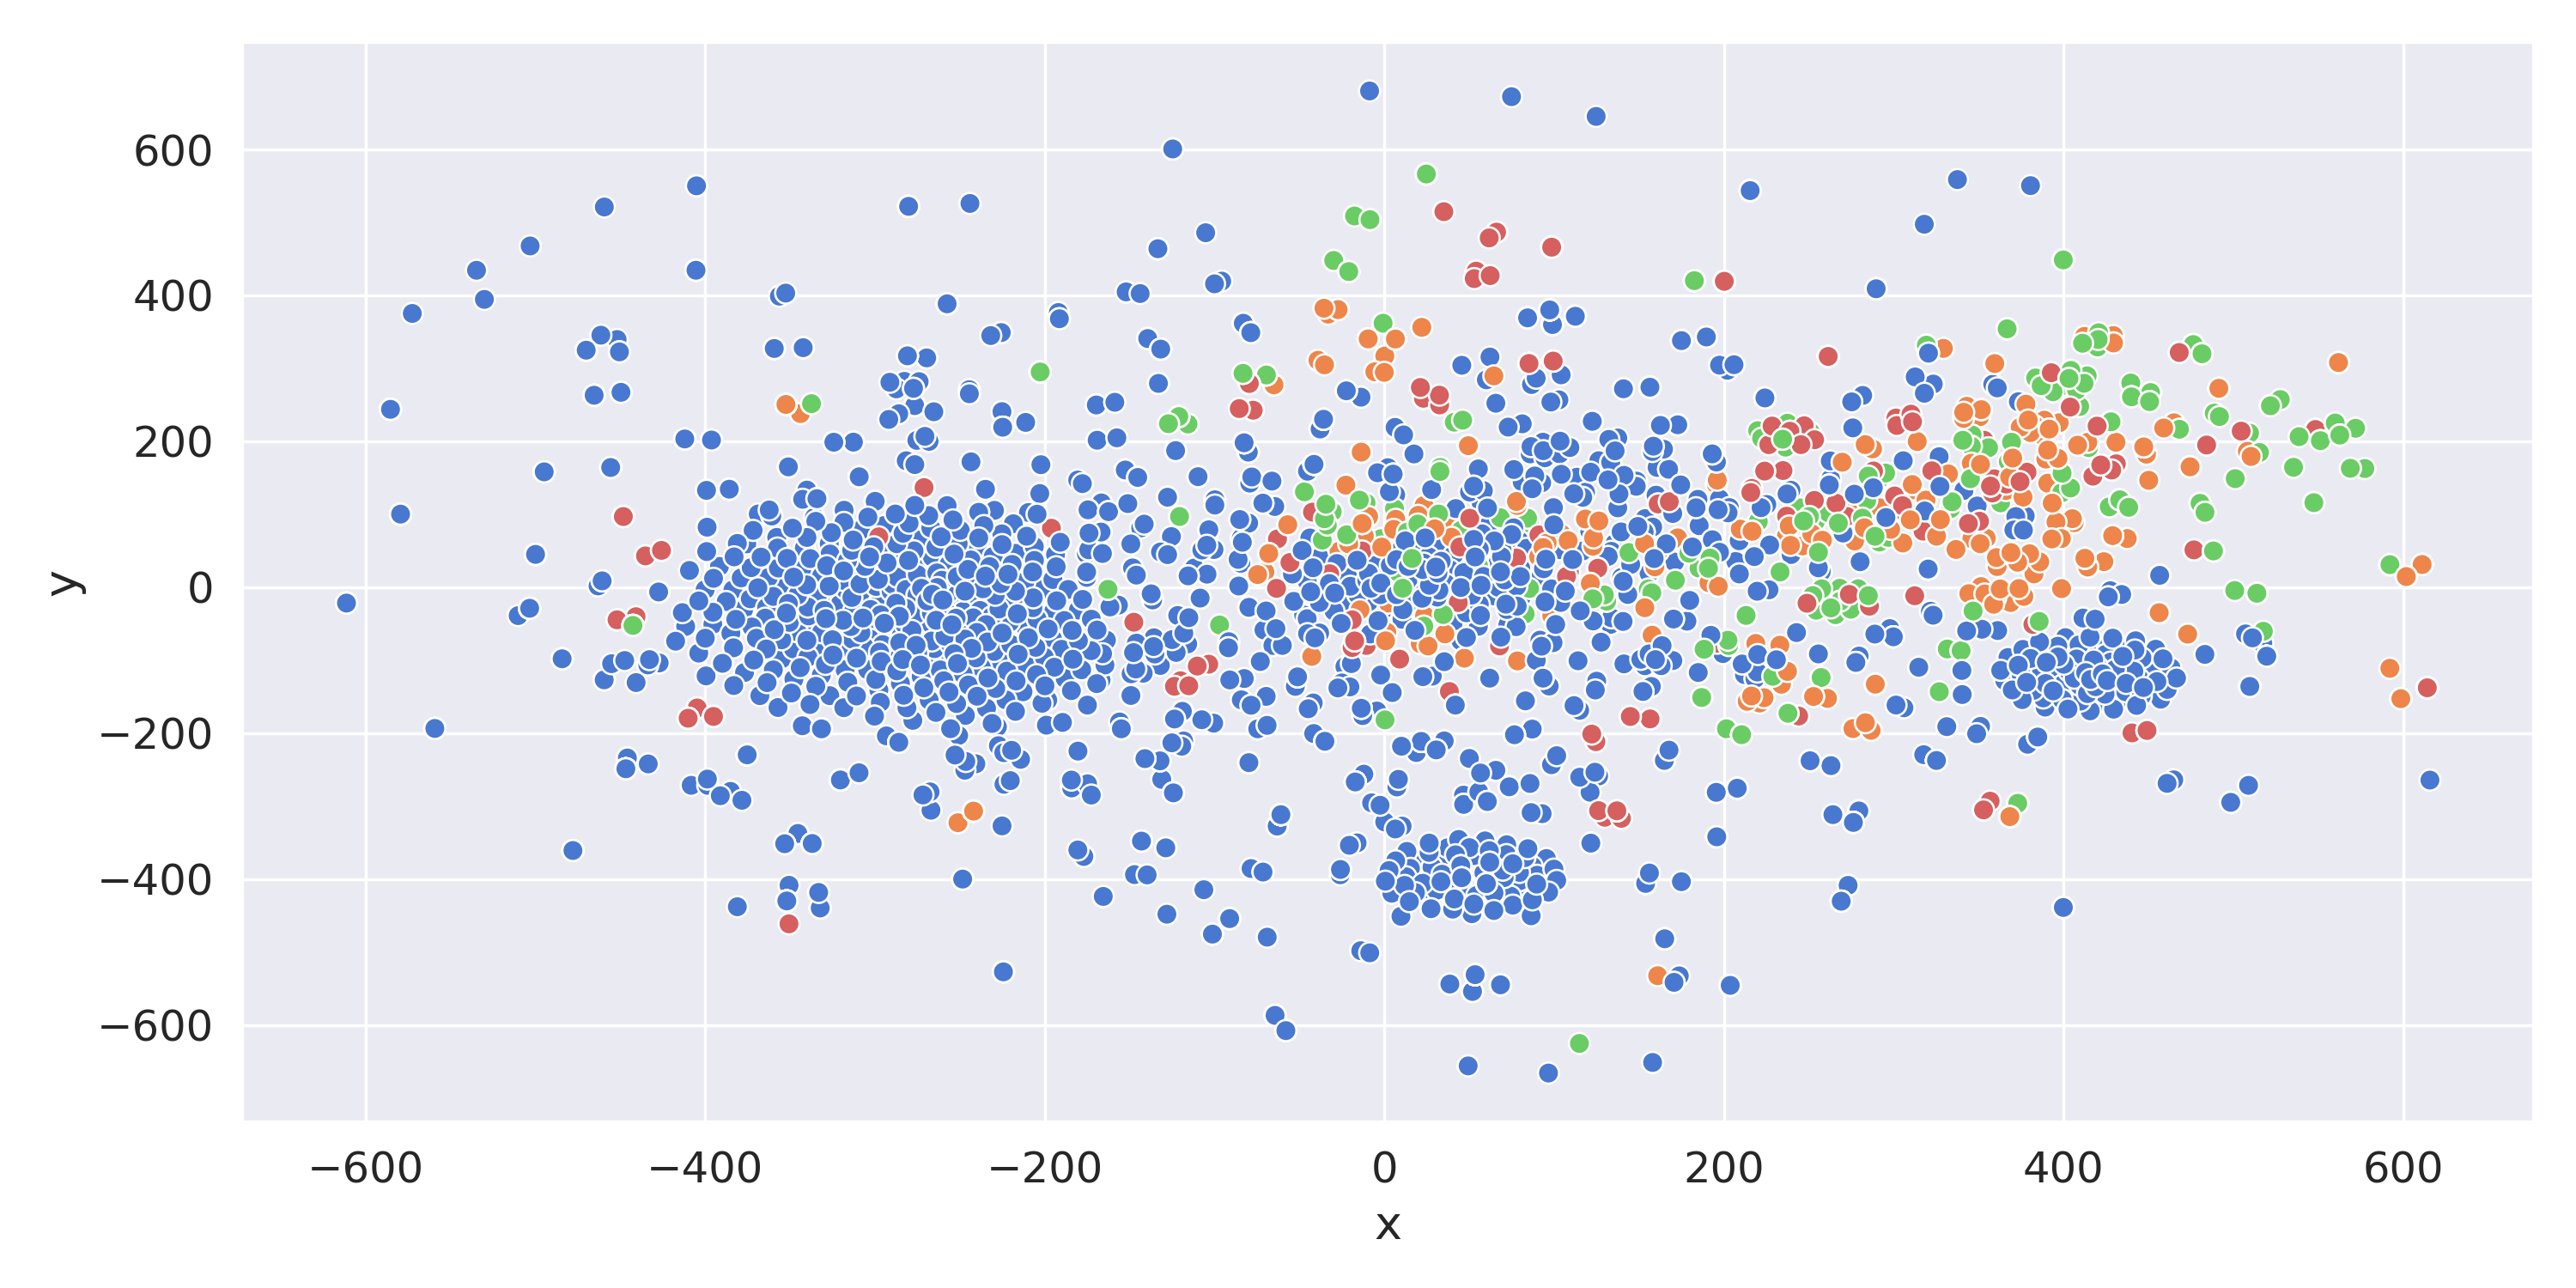
\includegraphics[width=\linewidth]{img/word2vec-embeddings.png}
  \caption{w2v\_trimmed}
  \label{fig:sfig1}
\end{subfigure}%
\begin{subfigure}{0.5\linewidth}
  \centering
  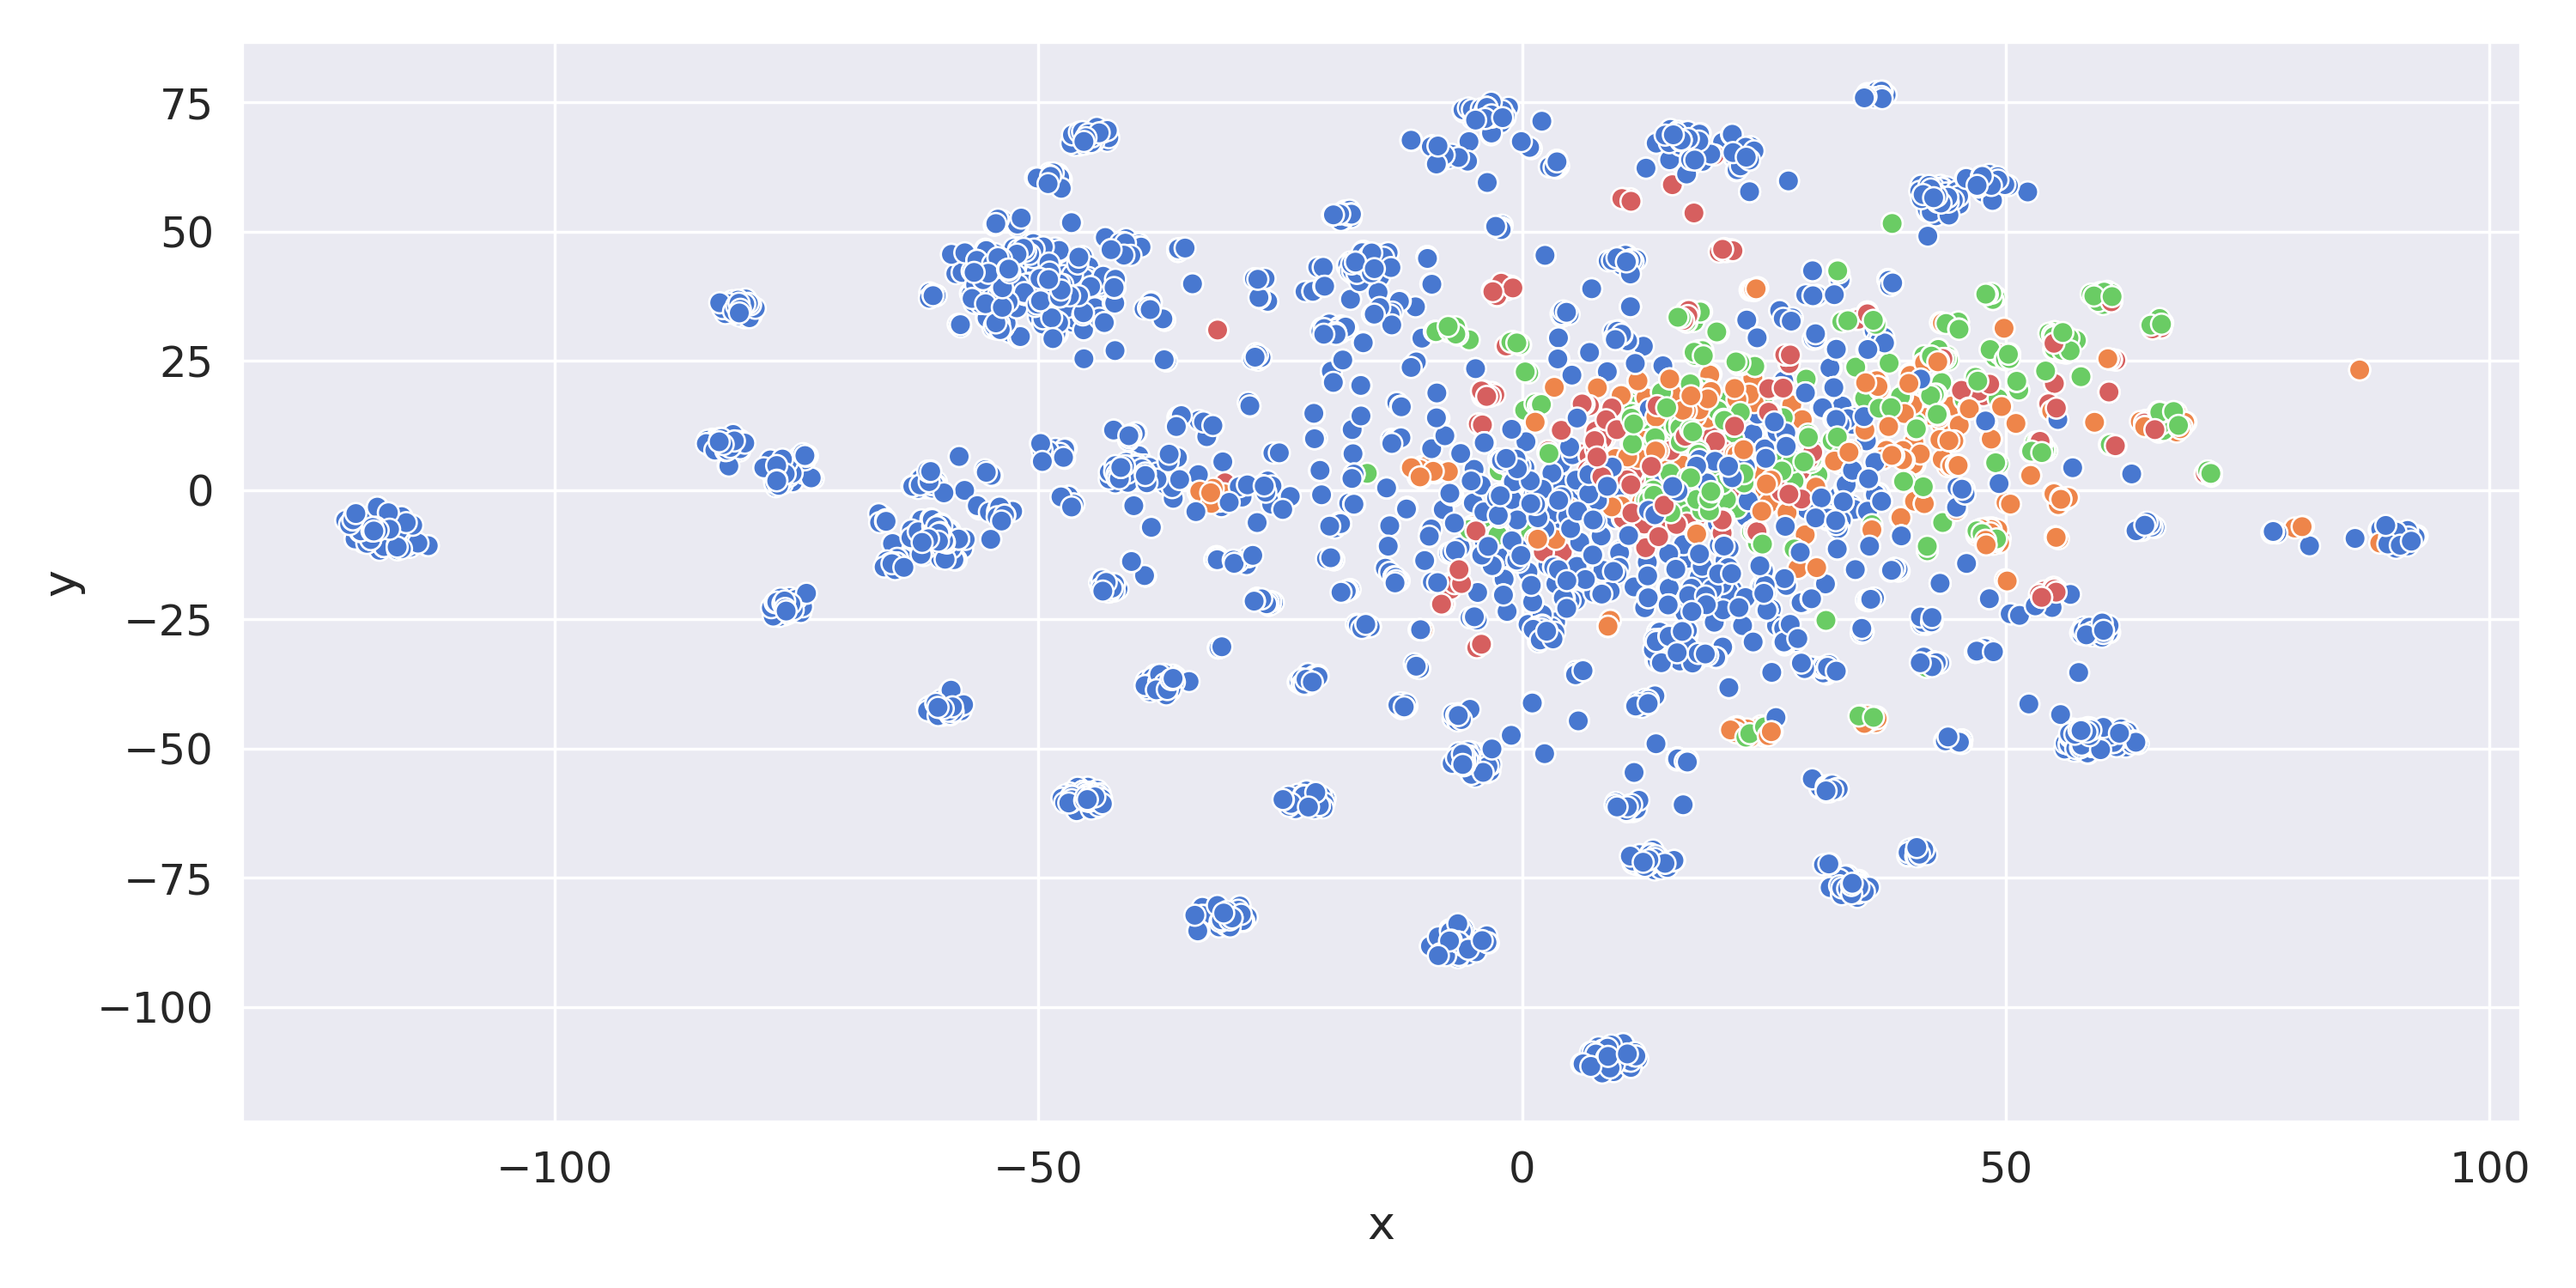
\includegraphics[width=\linewidth]{img/elmo-embeddings.png}
  \caption{ELMo}
  \label{fig:sfig2}
\end{subfigure}\\
\begin{subfigure}{0.5\linewidth}
  \centering
  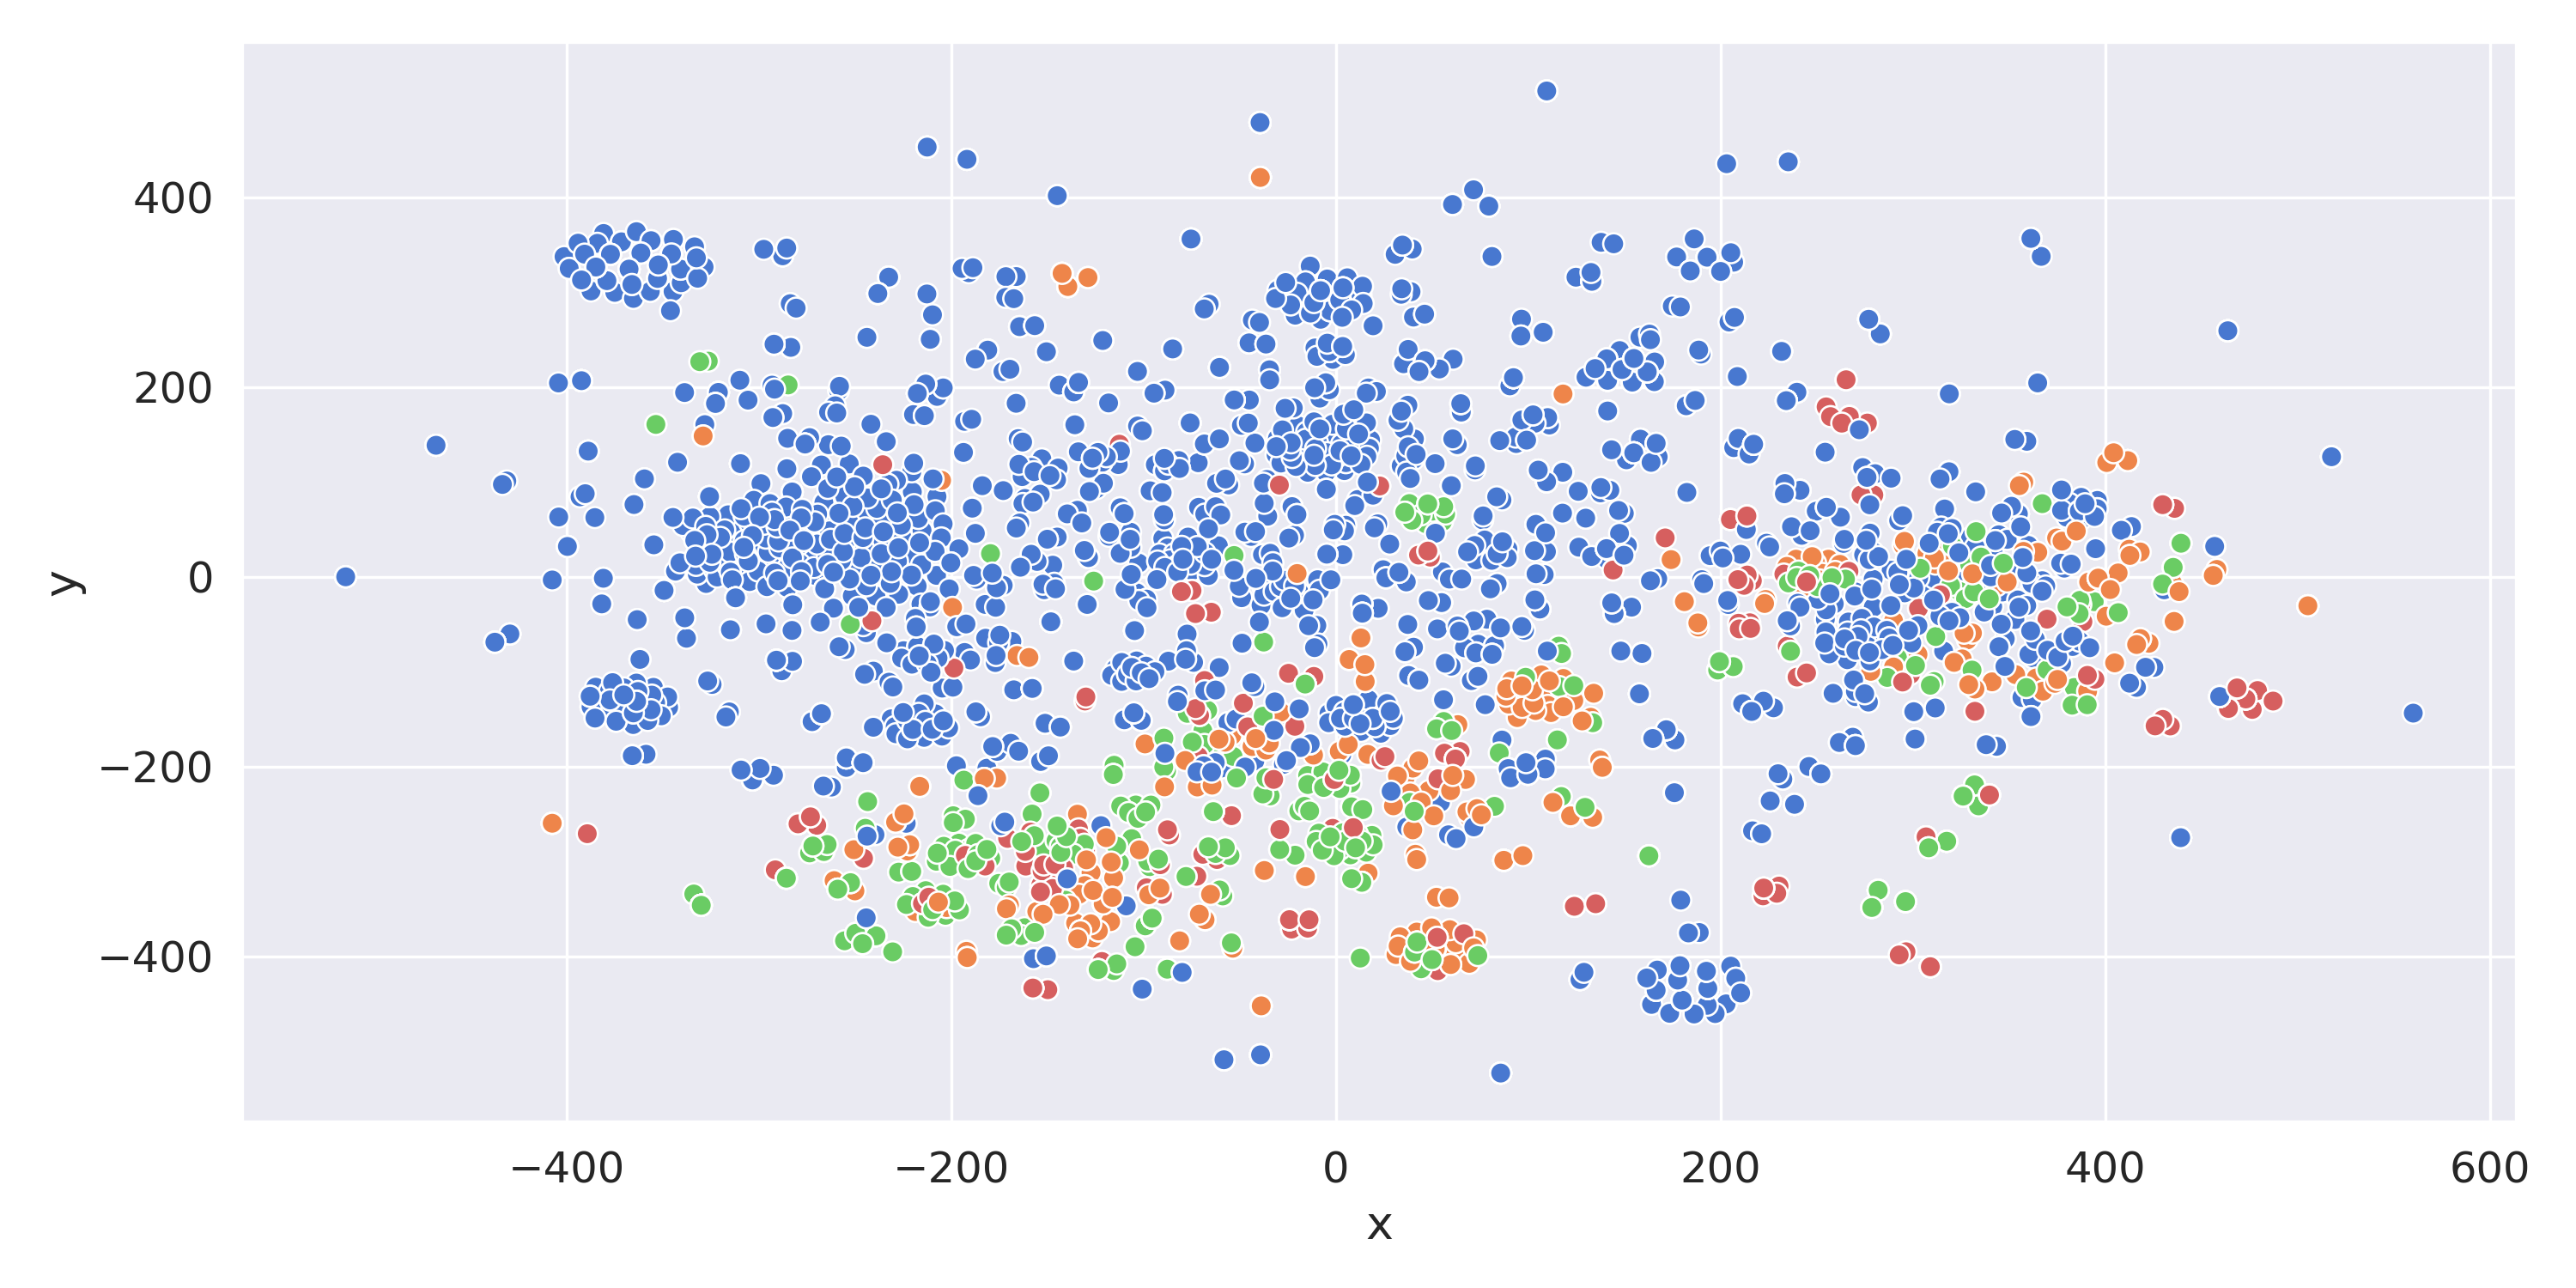
\includegraphics[width=\linewidth]{img/bert-embeddings.png}
  \caption{BERT}
  \label{fig:sfig2}
\end{subfigure}%
\begin{subfigure}{0.5\linewidth}
  \centering
  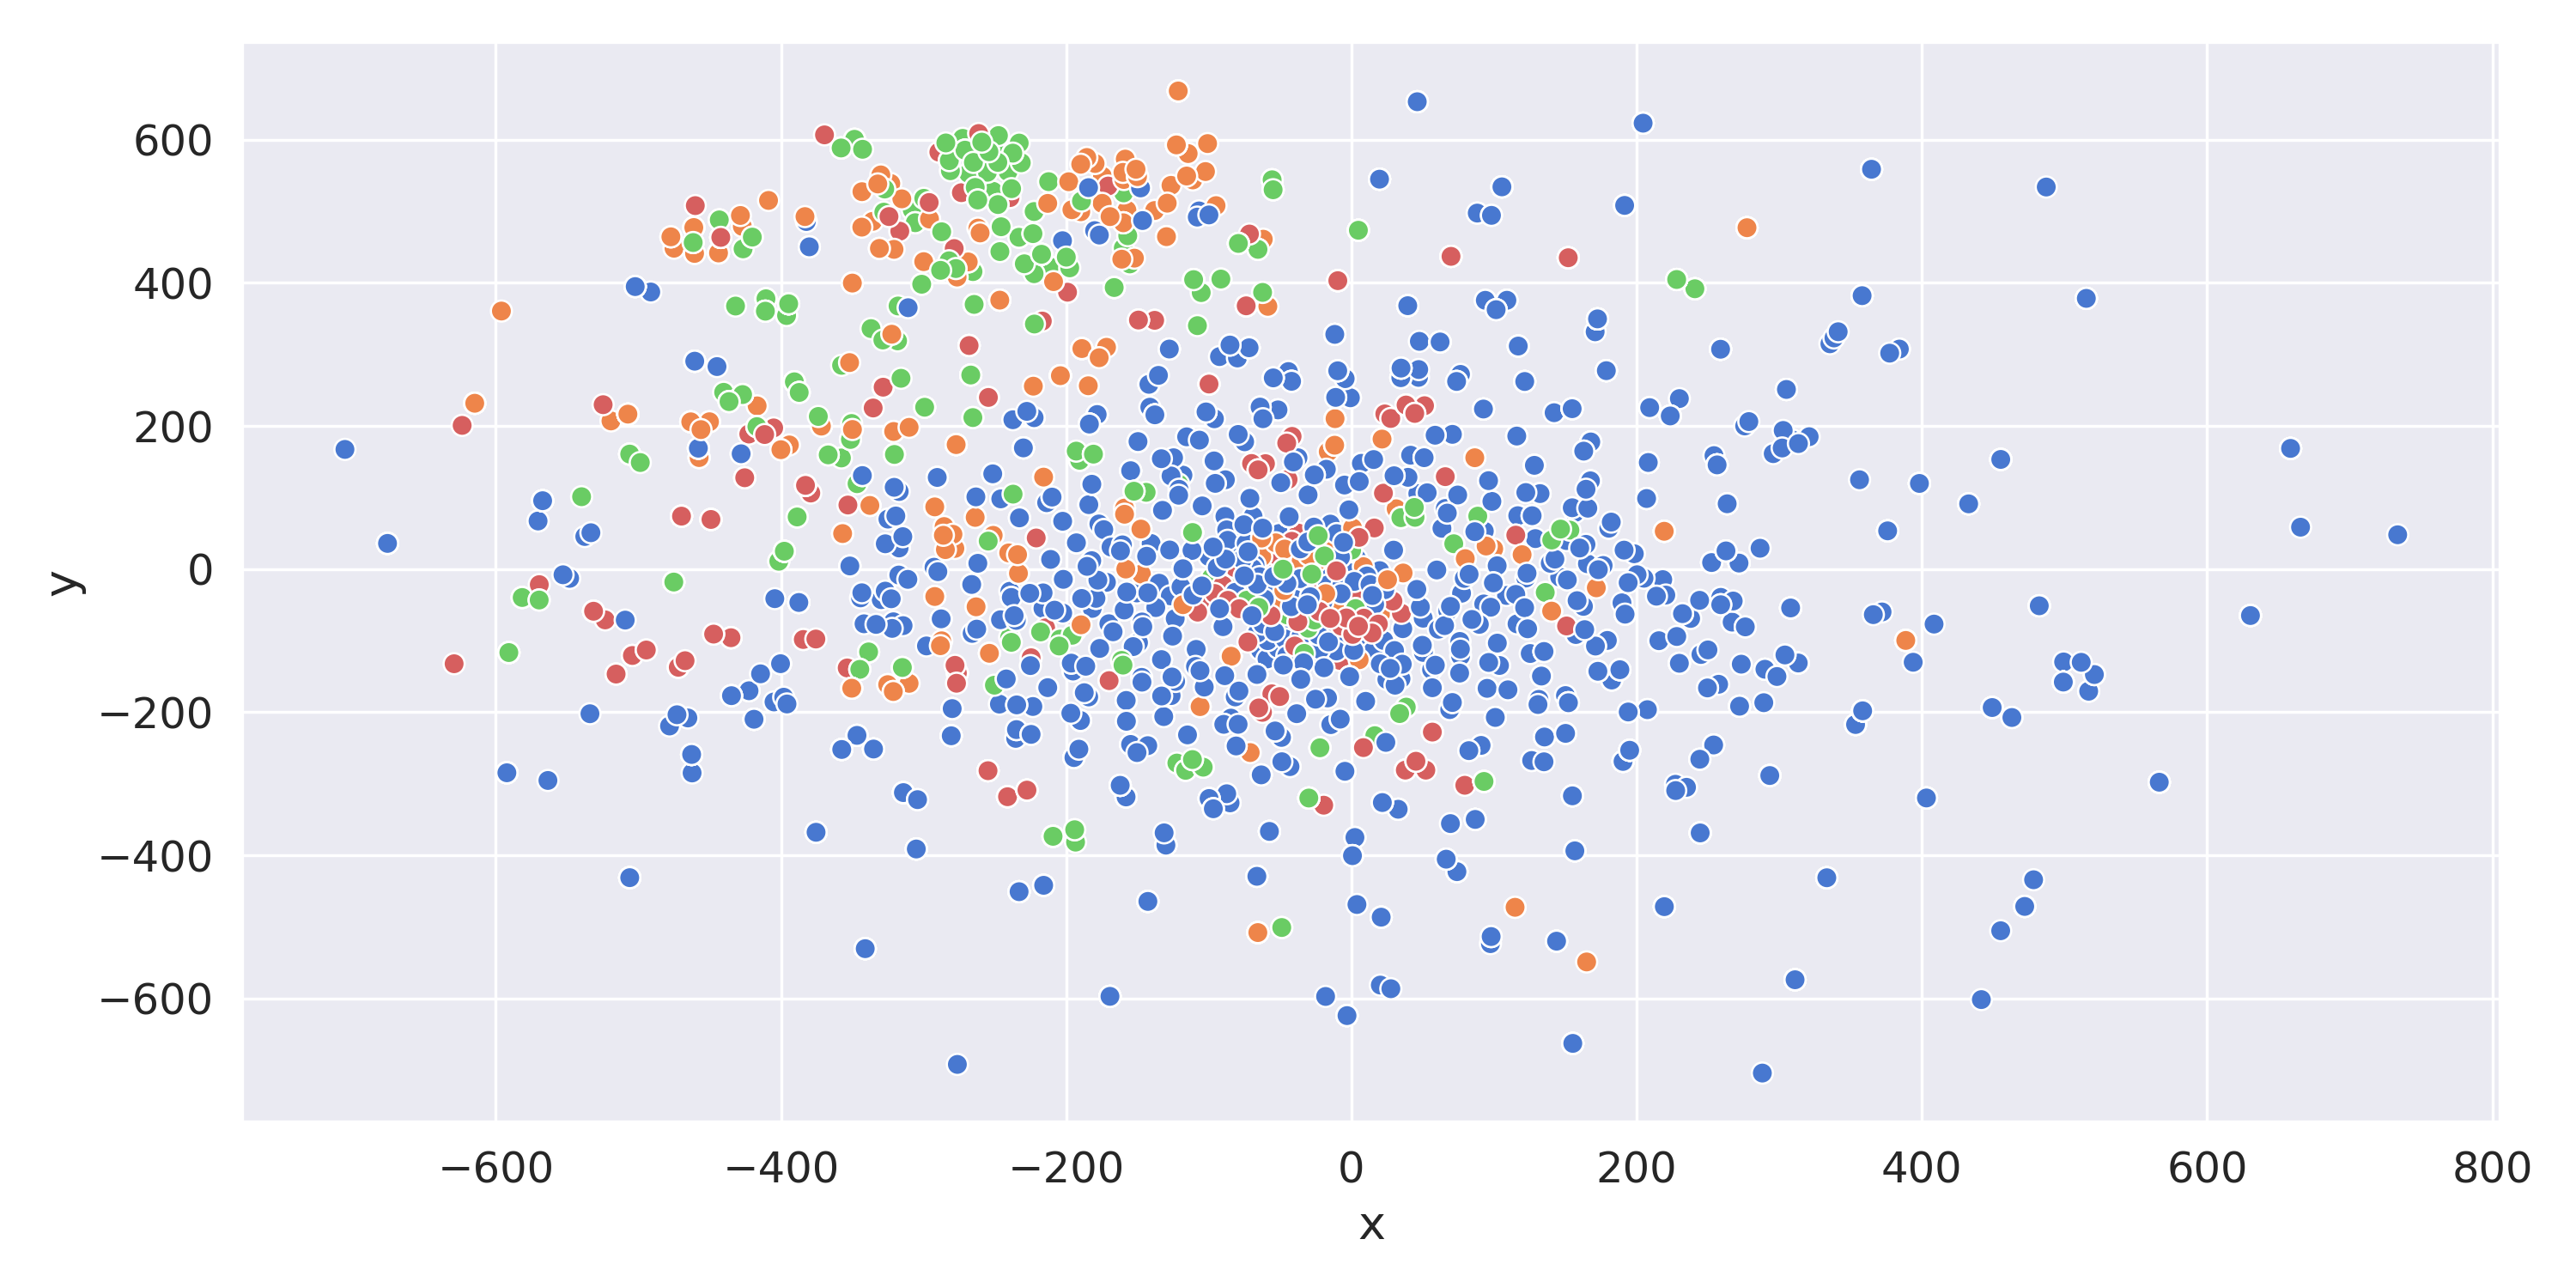
\includegraphics[width=\linewidth]{img/conceptnet-embeddings.png}
  \caption{ConceptNet}
  \label{fig:sfig2}
\end{subfigure}
\caption{These plots show the embeddings representation of four major concepts of the training dataset. Namely, \textit{movie.name} (blue), \textit{actor.name} (orange), \textit{producer.name} (red) and \textit{director.name} (green). We can clearly see how some embeddings enable nicer clusters for some concepts. 
}
\label{fig:fig-emb}
\end{figure*}


\subsection{BERT}

\textbf{BERT (Bidirectional Encoder Representations from Transformers)} \cite{devlin2018bert} is a relatively new language representation model released in 2019. It pre-trains deep bidirectional representations from unlabeled texts by exploiting both the left and right context. The model is a multi-layer bidirectional Transformer encoder. The authors state that this new representation solves the previous limitations of pre-trained models (e.g., ELMo). They argue that the standard LMs are unidirectional, thus limiting the kind of architectures which can be used during training. They also state that other pre-trained embeddings like ELMo are just shallow bidirectional since they use several separate models to capture the left and right context.
There are two steps in the BERT framework: \textit{pre-training} and \textit{fine-tuning}. During the first phase, the model is trained on unlabeled data over two separate unsupervised training tasks: \textit{Masked LM} and \textit{Next Sentence Prediction (NSP)}.  The Masked LM task consists of predicting some words of the given input phrase which are masked beforehand.  This would enable to train a real deep bidirectional representation since bidirectional conditioning on standard LM is not possible. The Next Sentence Prediction (NSP) consists of predicting relationships between sentences which are usually not captured by LM. 
During the fine-tuning phase, the model is initialized with the pre-trained parameters obtained in the previous stage and it is fine-tuned on the desired task. 
In our work, we used a pre-trained BERT model\footnote{\url{https://pypi.org/project/bert-embedding/}} to get the word embeddings directly without doing the fine-tuning phase. More specifically, the BERT model used was pre-trained on the BookCorpus \footnote{\url{https://yknzhu.wixsite.com/mbweb}} and English Wikipedia. The embedding dimension was 768.  

\begin{table*}[t]
\centering
\resizebox{\textwidth}{!}{%
\begin{tabular}{@{}|l|l|l|l|l|l|l|l|@{}}
\hline\textbf{Model} & \textbf{Hidden} & \textbf{Epochs} & \textbf{Batch} & \textbf{Lr} & \textbf{Drop rate} & \textbf{Emb} & \textbf{Min} $F_1$ / \textbf{Mean} $F_1$ / \textbf{Best} $F_1$ \\ \hline 
LSTM & 200 & 15 & 20 & 0.001& 0.7& w2v\_trimmed&\begin{tabular}[c]{@{}lll@{}}81.88 & 83.17 & 84.35\\ 
82.23 & \textbf{ 83.35 } & 84.22\\ 
\end{tabular} \\ \hline 
LSTM & 200 & 15 & 20 & 0.001& 0.7& ConceptNet&\begin{tabular}[c]{@{}lll@{}}81.58 & 82.49 & 83.75\\ 
81.78 & \textbf{ 82.94 } & 84.11\\ 
\end{tabular} \\ \hline 
LSTM & 200 & 30 & 20 & 0.001& 0.7& BERT&\begin{tabular}[c]{@{}lll@{}}77.06 & 79.10 & 81.39\\ 
80.51 & \textbf{ 82.13 } & 83.66\\ 
\end{tabular} \\ \hline 
LSTM & 200 & 30 & 20 & 0.001& 0.7& ELMo&\begin{tabular}[c]{@{}lll@{}}81.77 & 82.65 & 83.48\\ 
83.77 & \textbf{ 84.40 } & 85.35\\ 
\end{tabular} \\ \hline 
LSTM & 200 & 30 & 20 & 0.001& 0.7& ELMo (fine tuned)&\begin{tabular}[c]{@{}lll@{}}75.19 & 82.29 & 85.14\\ 
82.88 & \textbf{ 84.47 } & 85.60\\ 
\end{tabular} \\ \hline 
LSTM-CRF & 200 & 10 & 1 & 0.001& 0.7& w2v\_trimmed&\begin{tabular}[c]{@{}lll@{}}84.85 & \textbf{ 85.70 } & 86.83\\ 
84.66 & 85.35 & 86.30\\ 
\end{tabular} \\ \hline 
LSTM-CRF & 200 & 10 & 1 & 0.001& 0.7& ConceptNet&\begin{tabular}[c]{@{}lll@{}}85.46 & \textbf{ 85.94 } & 86.52\\ 
85.49 & 85.83 & 86.51\\ 
\end{tabular} \\ \hline 
LSTM-CRF & 200 & 20 & 1 & 0.001& 0.7& BERT&\begin{tabular}[c]{@{}lll@{}}82.33 & 83.73 & 84.95\\ 
83.10 & \textbf{ 83.83 } & 84.98\\ 
\end{tabular} \\ \hline 
LSTM-CRF & 200 & 20 & 1 & 0.001& 0.7& ELMo&\begin{tabular}[c]{@{}lll@{}}84.50 & \textbf{ 85.53 } & 86.39\\ 
84.12 & 85.29 & 86.29\\ 
\end{tabular} \\ \hline 
LSTM-CRF & 200 & 10 & 1 & 0.001& 0.7& ELMo (fine tuned)&\begin{tabular}[c]{@{}lll@{}}84.34 & 85.72 & 86.56\\ 
83.96 & \textbf{ 85.81 } & 86.81\\ 
\end{tabular} \\ \hline 
\end{tabular}}
\caption{Evaluation results of the various models. Each model is bidirectional. The performances were obtained by recording the results for 25 runs by varying the initialization parameters of the models and by keeping their hyperparameters fixed. The rightmost column is divided as such: the first line shows the results without any improvements and the second line shows the results by adding the character convolution (CHAR) and the NER and POS tagging features. The \textbf{bold} values indicate the best result for that particular embedding.
}
\label{tab:final-results}
\end{table*}

\section{Data Analysis}

We evaluated our solutions by using the NL2SparQL4NLU dataset \footnote{\url{https://github.com/esrel/NL2SparQL4NLU}}. It corresponds to the MOVIE dataset of the original paper. It includes sentences taken from the movie domain (e.g., ``\textit{trailer for star wars a new hope}"). The dataset contains 3338 and 1084 sentences for the train and test set respectively. The dictionary size (\# of unique tokens) is of 1728 (train) and 1039 (test) with an OOV rate between the datasets of 24\%. The average sentence length is 6.42 (train) and 6.52 (test). We have a total of 23 concepts (with 43 concepts in IOB format). Each word was also POS tagged and there are 50 different tags between the training and test set (taken from the Tree Tagger POS list\footnote{\url{https://courses.washington.edu/hypertxt/csar-v02/penntable.html}}).
We generated a new dataset by analyzing each sentence using a Named Entity Recognition (NER) tool, spaCy\footnote{\url{https://spacy.io/}}. It found 398 (1,86\%)  and 169 (2,37\%) entities inside the training and test set respectively. These entities were of 9 different types\footnote{\url{https://spacy.io/api/annotation\#named-entities}}.

\subsection{Embeddings Analysis}
We evaluated also the various embeddings using the \textit{embedding coverage} metric (namely, how many words in the dataset dictionary can be found in the embedding matrix) and we compared it with the embeddings used in the original work. With the default embeddings (w2v\_trimmed), the coverage is 96.18\% (66 words not recognized) while with ConceptNet the coverage is 91.90\% (140 words not recognized). For BERT and ELMo models we performed a visual analysis instead by using dimensionality reduction techiques. More specifically, we used \textit{t-SNE} \cite{Maaten2008VisualizingDU} to reduce the dimensionality of the BERT/ELMo embeddings down to 2-dimensional data points and then we plotted the results for the four most represented concepts in the dataset. See Figure \ref{fig:fig-emb} for the results. It is possible to notice how the default embeddings, ELMo and BERT produce nice clusters for the \textit{movie.name} category. The other categories are slightly mixed together which is expected. For instance, \textit{actor.name} and \textit{director.name} may end up with the same embedding since a person name can be referring both to an actor and to a movie director.
BERT and ELMo should be able to discriminate between them since they can exploit the context, but the lack of clusters could be caused by the \textit{t-SNE} reduction.
Ultimately, ConceptNet does not produce significant clusters (apart from a small one composed by \textit{director.name} elements). This however could be again caused by the \textit{t-SNE} reduction.

\begin{figure*}[t]
\begin{subfigure}{0.5\linewidth}
  \centering
  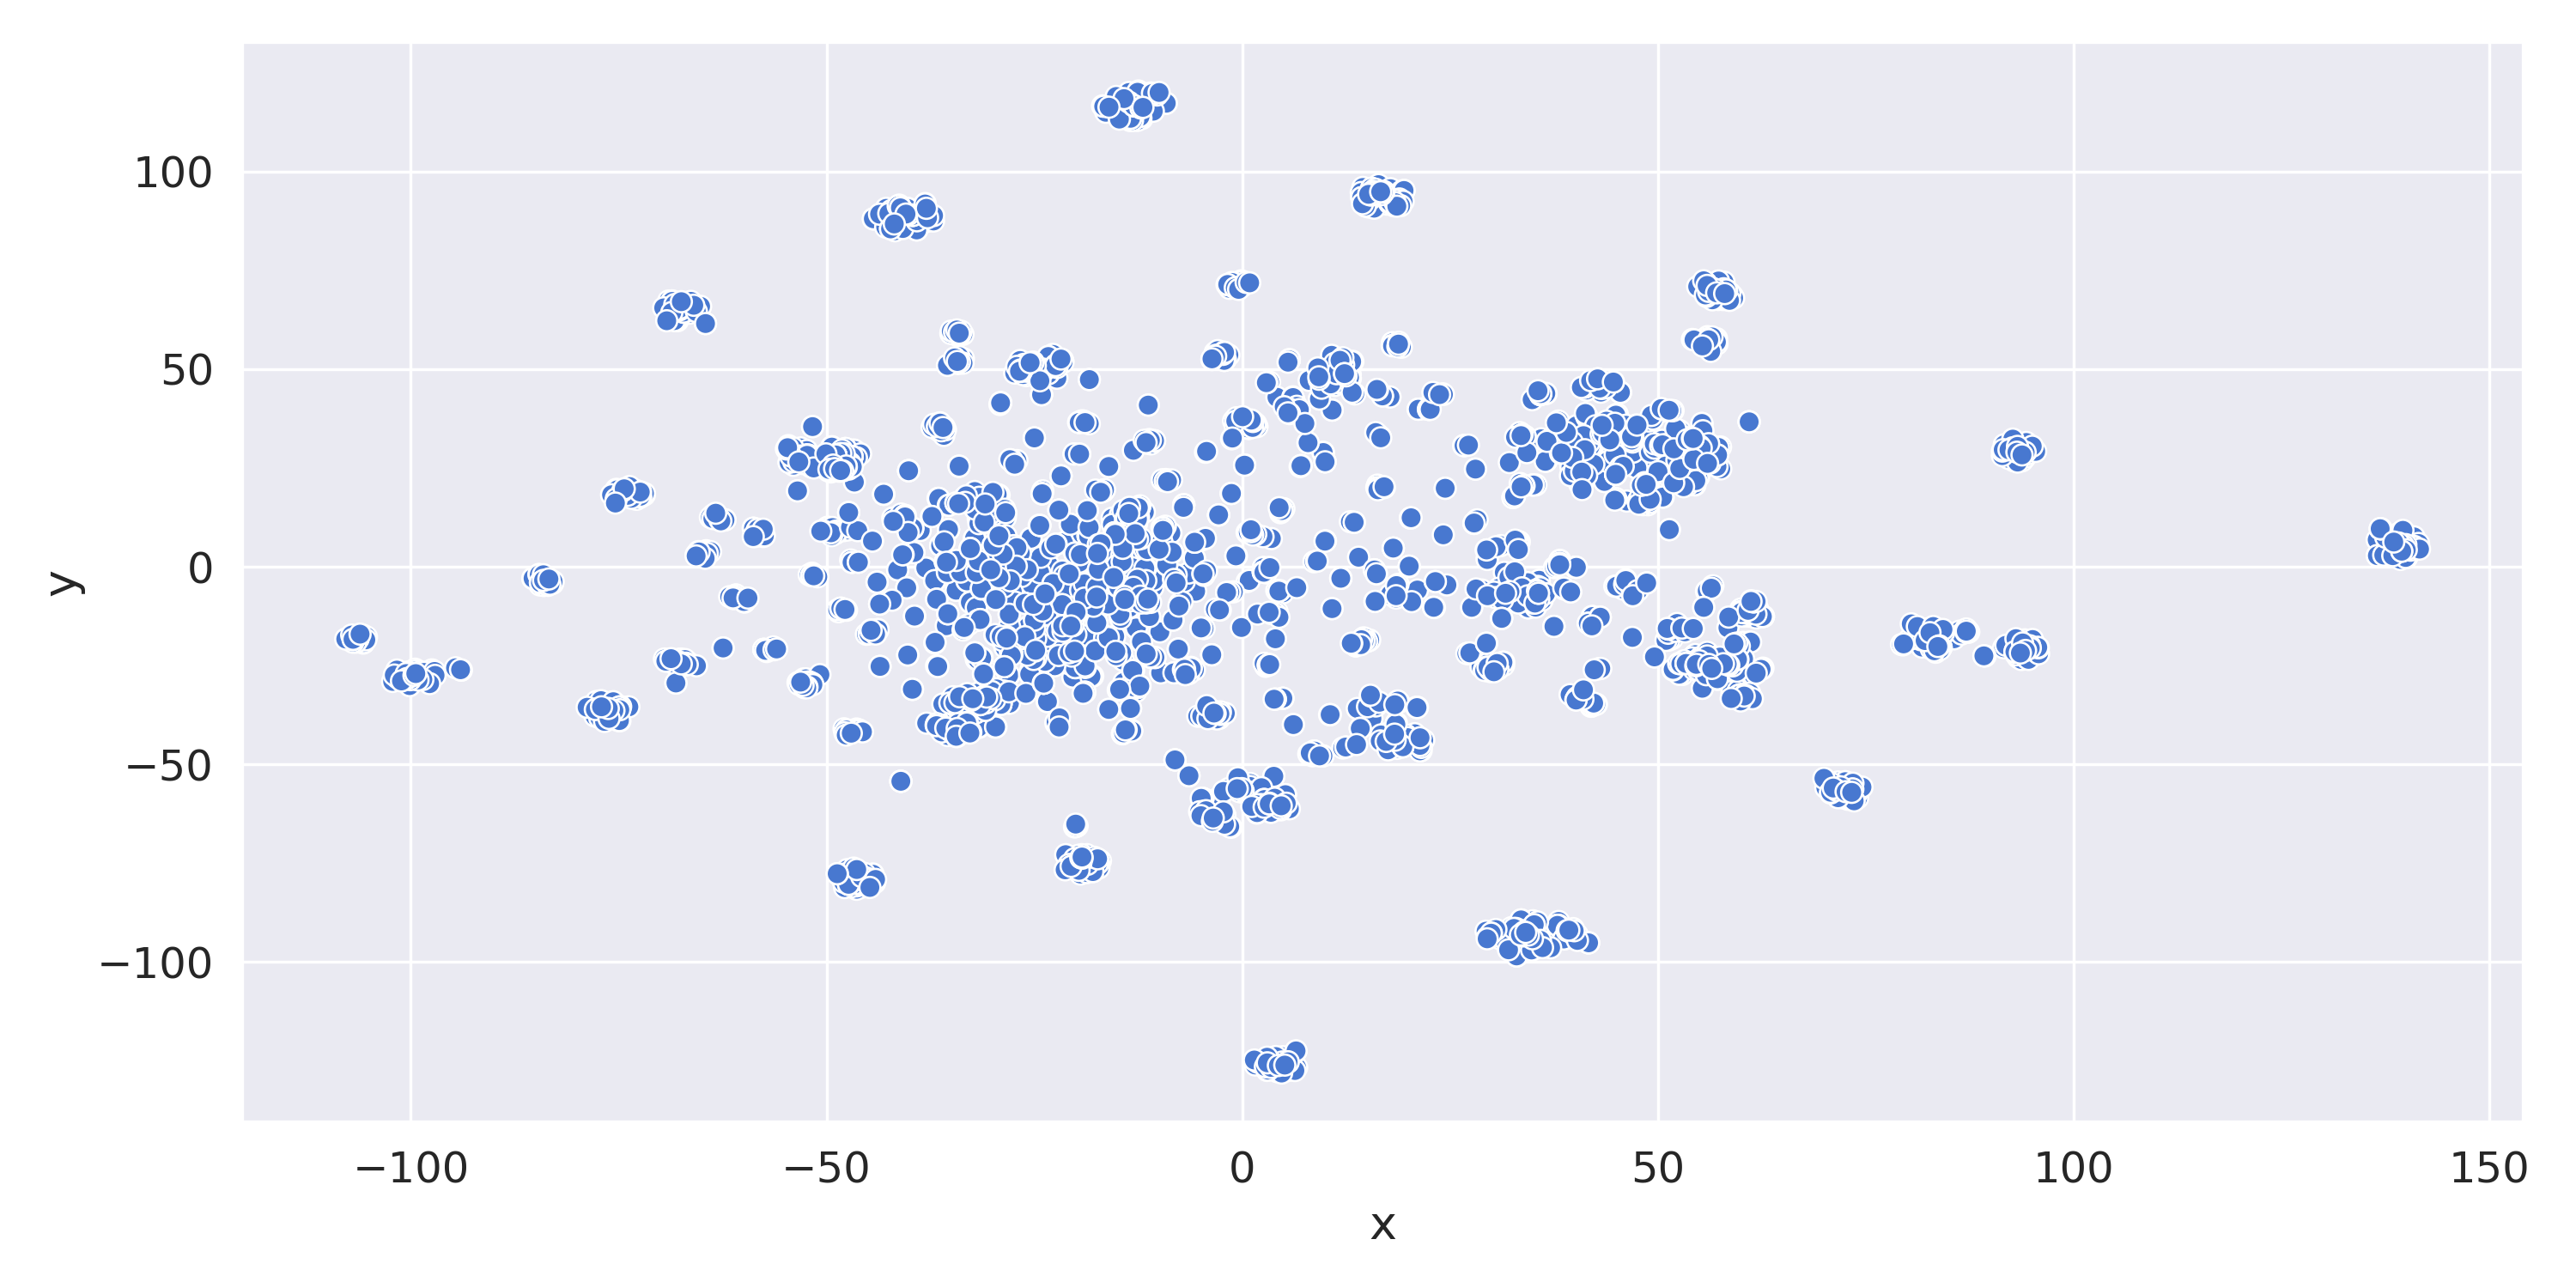
\includegraphics[width=\linewidth]{img/elmo-embeddings-not-trained-2D.png}
  \caption{Default ELMo Embeddings (\textit{movie.name} only)}
  \label{fig:sfig1}
\end{subfigure}%
\begin{subfigure}{0.5\linewidth}
  \centering
  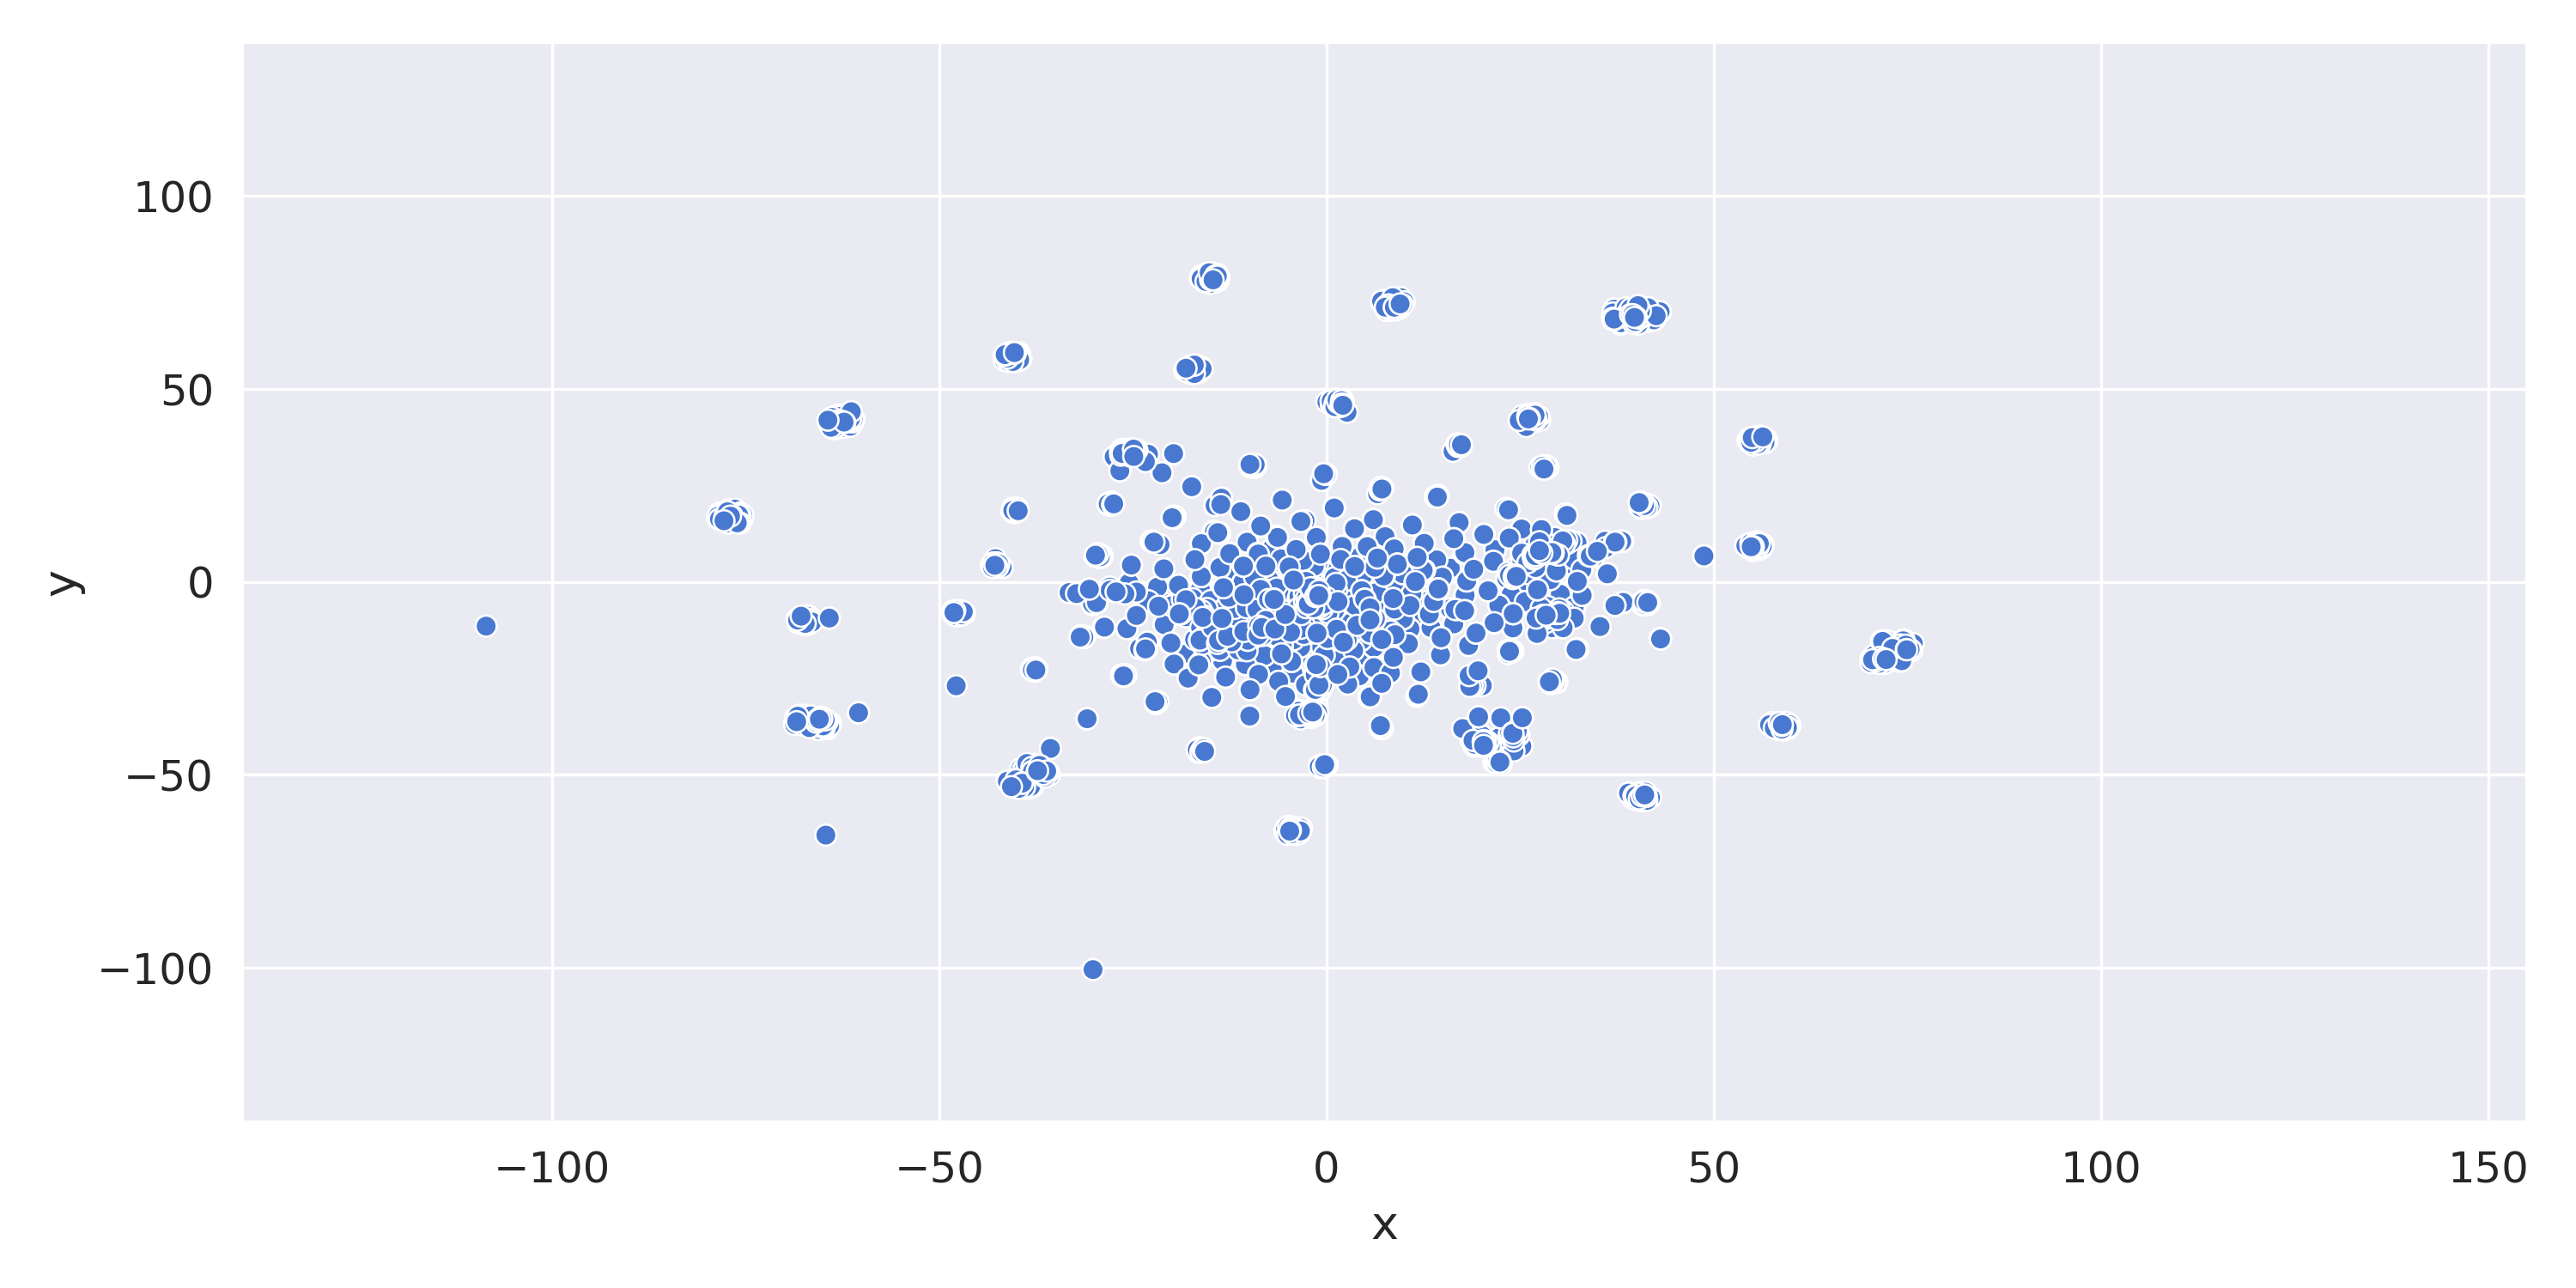
\includegraphics[width=\linewidth]{img/elmo-embeddings-trained-2D.png}
  \caption{Fine-Tuned ELMo Embeddings (\textit{movie.name} only).}
  \label{fig:sfig2}
\end{subfigure}%\\
%\begin{subfigure}{0.5\linewidth}
%  \centering
%  \includegraphics[width=\linewidth]{img/elmo-%embeddings-not-trained.png}
%  \caption{Averaged ELMo Embeddings 3D}
%  \label{fig:sfig1}
%\end{subfigure}%
%\begin{subfigure}{0.5\linewidth}
%  \centering
%  \includegraphics[width=\linewidth]{img/elmo-%embeddings-trained.png}
%  \caption{Learned Elmo Embeddings 3D %(\textit{movie.title} only).}
%  \label{fig:sfig2}
%\end{subfigure}
\caption{These plots show how the embeddings clustering for the \textit{movie.name} concept changes between the averaged version and the fine-tuned one. Fine-tuning the weights gives importance on the higher layers which capture context-dependent aspects of word meaning and therefore they help to produce better clustering.}
\label{fig:fine-tuned-emb}
\end{figure*}

\section{Experiments}

We evaluated the models by doing a hyperparameter search by starting from the values used in the original work. We tried to find the hyperparameter combination which maximizes the mean $F_1$ score over the test dataset. The final results can be seen in Table \ref{tab:final-results}.
When using a classical LSTM model, it is clear that by combining the character representation (CHAR) and the additional features (POS+NER) we obtain better results than the default baseline. This happens regardless of the embeddings employed. Moreover, the ELMo embeddings provide better performances than the other competitors. 
The BERT embeddings give instead less performing results (more than 3\% difference between the $F_1$ mean baseline in some cases). \textit{However, it seems that using different embeddings does improve the baseline.}
When using the LSTM-CRF we obtained slightly different results. The LSTM-CRF generally outperforms the simple LSTM model, but here adding the CHAR+NER+POS features gives good results only when using the fine-tuned ELMo embeddings or BERT. By employing ConceptNet or the default embeddings we obtain a better $F_1$ score without using those features (even if the difference is minimal).
By using LSTM-CRF and ELMo (fine-tuned) we were able to reach the highest $F_1$ score of 86.81 over the various embeddings (the baseline model reaches a maximum of 86.83). Ultimately, the best combination overall with a mean $F_1$ value of 85.94 is obtained by using the ConceptNet embeddings without additional features and the LSTM-CRF model. All these results surpass the previous baseline obtained with the WFST (83.73).
The models were written in Python and PyTorch by forking from the previous project\footnote{\url{https://github.com/fruttasecca/concept-tagging-with-neural-networks}} and both the code and the dataset are available on Github\footnote{\url{https://github.com/geektoni/concept-tagging-nn-spacy}}.

\subsection{Effects of Embeddings Fine-Tuning}

Next we focused on analyzing the used embeddings by focalizing on ELMo which gave the most interesting results. We studyied the visual differences between the fine-tuned and averaged ELMo embeddings. We also evaluated the SSE (Sum of Squared Errors) of the generated clusters for certain concepts. By fine-tuning the ELMo weightings, it is possible to generate slightly better ``concept clusters" in the embedding space. Figure \ref{fig:fine-tuned-emb} shows an example. 
We also saw an SSE error reduction of almost 50\% with the fine-tuned version (from 13490936.61 to 7267435.40) when considering the \textit{movie.name} concept. This is beneficial because a Neural Network learns how to divide the features space such to separate with hyperplanes each concept. Then we just need to check where the representation of my token lies to assign a concept.  However, we noticed that, since our dataset is imbalanced (the concepts \textit{O} and \textit{movie.title} takes 80\% of the total) only the clusters of the majority classes will be improved. This is corroborated by the fact that by analyzing the \textit{confusion matrices} of the fine-tuned ELMo models (both LSTM and LSTM-CRF) it is possible to see how the accuracy of the majority concepts increases slightly while the accuracy of the other concepts degrades. See Table \ref{tab:elmo-comp} for a comparison between the ELMo versions. We can conclude that fine-tuning pre-trained contextual embeddings is always advisable. 

\begin{table*}[]
\centering
\resizebox{\textwidth}{!}{%
\begin{tabular}{l|l|l|l|l|l|l|l|}
\cline{2-8}
 & \textbf{O} & \textbf{movie.name} & \textbf{director.name} & \textbf{actor.name} & \textbf{producer.name} & \textbf{movie.language} & \textbf{movie.release\_date} \\ \hline
\multicolumn{1}{|l|}{\textbf{Averaged ELMo}} & 0.99584898 & 0.94475655 & 0.85628743 & 0.89855072 & 0.96330275 & \textbf{0.92592593} & \textbf{0.94117647} \\
\multicolumn{1}{|l|}{\textbf{Fine-Tuned ELMo}} & \textbf{0.99625468} & \textbf{0.96190476} & \textbf{0.87647059} & \textbf{0.91724138} & \textbf{0.98181818} & 0.84745763 & 0.90410959 \\ \hline
\end{tabular}%
}
\caption{Given the top-seven concepts from the test dataset, we compute the tagging accuracy when using the LSTM-CRF and the CHAR+POS+NER features. The first five concepts appear more than 2\% over the entire dataset, while the last two appear less than 1\%. It is possible to see how the performances increase for the first fìive when using the fine-tuned ELMo, while the other two accuracies decrease with respect to the averaged ELMo.}
\label{tab:elmo-comp}
\end{table*}


\section{Conclusion}
The experiments gave us new insights about the usage of embeddings for obtaining state-of-the-art performances on concept tagging tasks. BERT and ELMo pre-trained models provide new embeddings obtained by looking at the entire phrase. However, they cannot be used directly out-of-the-box but they need to be fine-tuned on the task at hand to be effective. This can be clearly seen by looking at the difference between the ELMo embeddings created by mere averaging of the layers and by learning instead the weights of the linear combination. We showed how ELMo fine-tuned embeddings provides certain advantages with respect to their not-tuned version. We think this is also the reason why BERT underperformed in some cases. We used an implementation which extracts directly the embeddings without going through the fine-tuning phase described in the original BERT paper. Therefore, the embeddings are not ``trained" to interpret the current concept tagging task and they lead to bad performances. We are aware of the issues which arise from our validation methods (in particular, \textit{t-SNE} \cite{wattenberg2016how}) but we believe they still provide useful information.
We presented also the impact of adding more features to the original model, more specifically, the POS tag and the NER entities. However, we did not see any important improvement. \textit{We thought that having extra information like the NER tags could have improved the performances of the models but it was not the case}. This happened for several reasons. For instance, one major problem we found with this method is related to the sparsity of the NER tagging. On over 21000 tokens, only 400~ were tagged with an entity definition (just the 1.9\%). This adds just too little discriminative power to the original model and therefore it does not produce any huge gain in performances.
In conclusion, we were able to surpass classical WFST methods and we were able to almost replicate the results of \citet{gobbi}. \textit{However, even by employing more advanced embeddings and new feature combinations, we were unable to generate significative improvements during the evaluation}.  
We think that the general issue that needs to be solved to get better results is the unbalanced dataset we are using. Some concepts are underrepresented (e.g., \textit{actor.type}, \textit{actor.nationality}, etc.) while others are present in large quantity (e.g., \textit{O} and \textit{movie.name}). The model will be pushed to learn to classify the majority classes while ignoring the rest. We believe that this problem can be solved by increasing the size of the dataset. This can be done either by gathering real-world examples or by generating \textit{synthetic sentences} by sampling from a statistical model trained on the original dataset. However, this task was left for future work.

\bibliography{acl2019}
\bibliographystyle{acl_natbib}

\end{document}
